%app overview
\subsection{Application Overview}
The ReVA application is an android mobile application designed to report vitals information of registered bedridden patients to registered subscribers (this includes the patients themselves). It is a tool meant to bridge the distance gap between caretaker and patient, allowing for real time vitals data to be monitored from any location with access to WiFi as well as trigger notifications when vitals stray from the norm. 

ReVA also has the functionality to display statistical and historical vitals information for long term monitoring of patient health. There is also an advice section that may be viewed for additional help. Advice may also be triggered based on notification alerts. 
%image of applications with numbers on buttons
\begin{figure}[ht!]
\centering
\begin{minipage}{.5\textwidth}
  \centering
  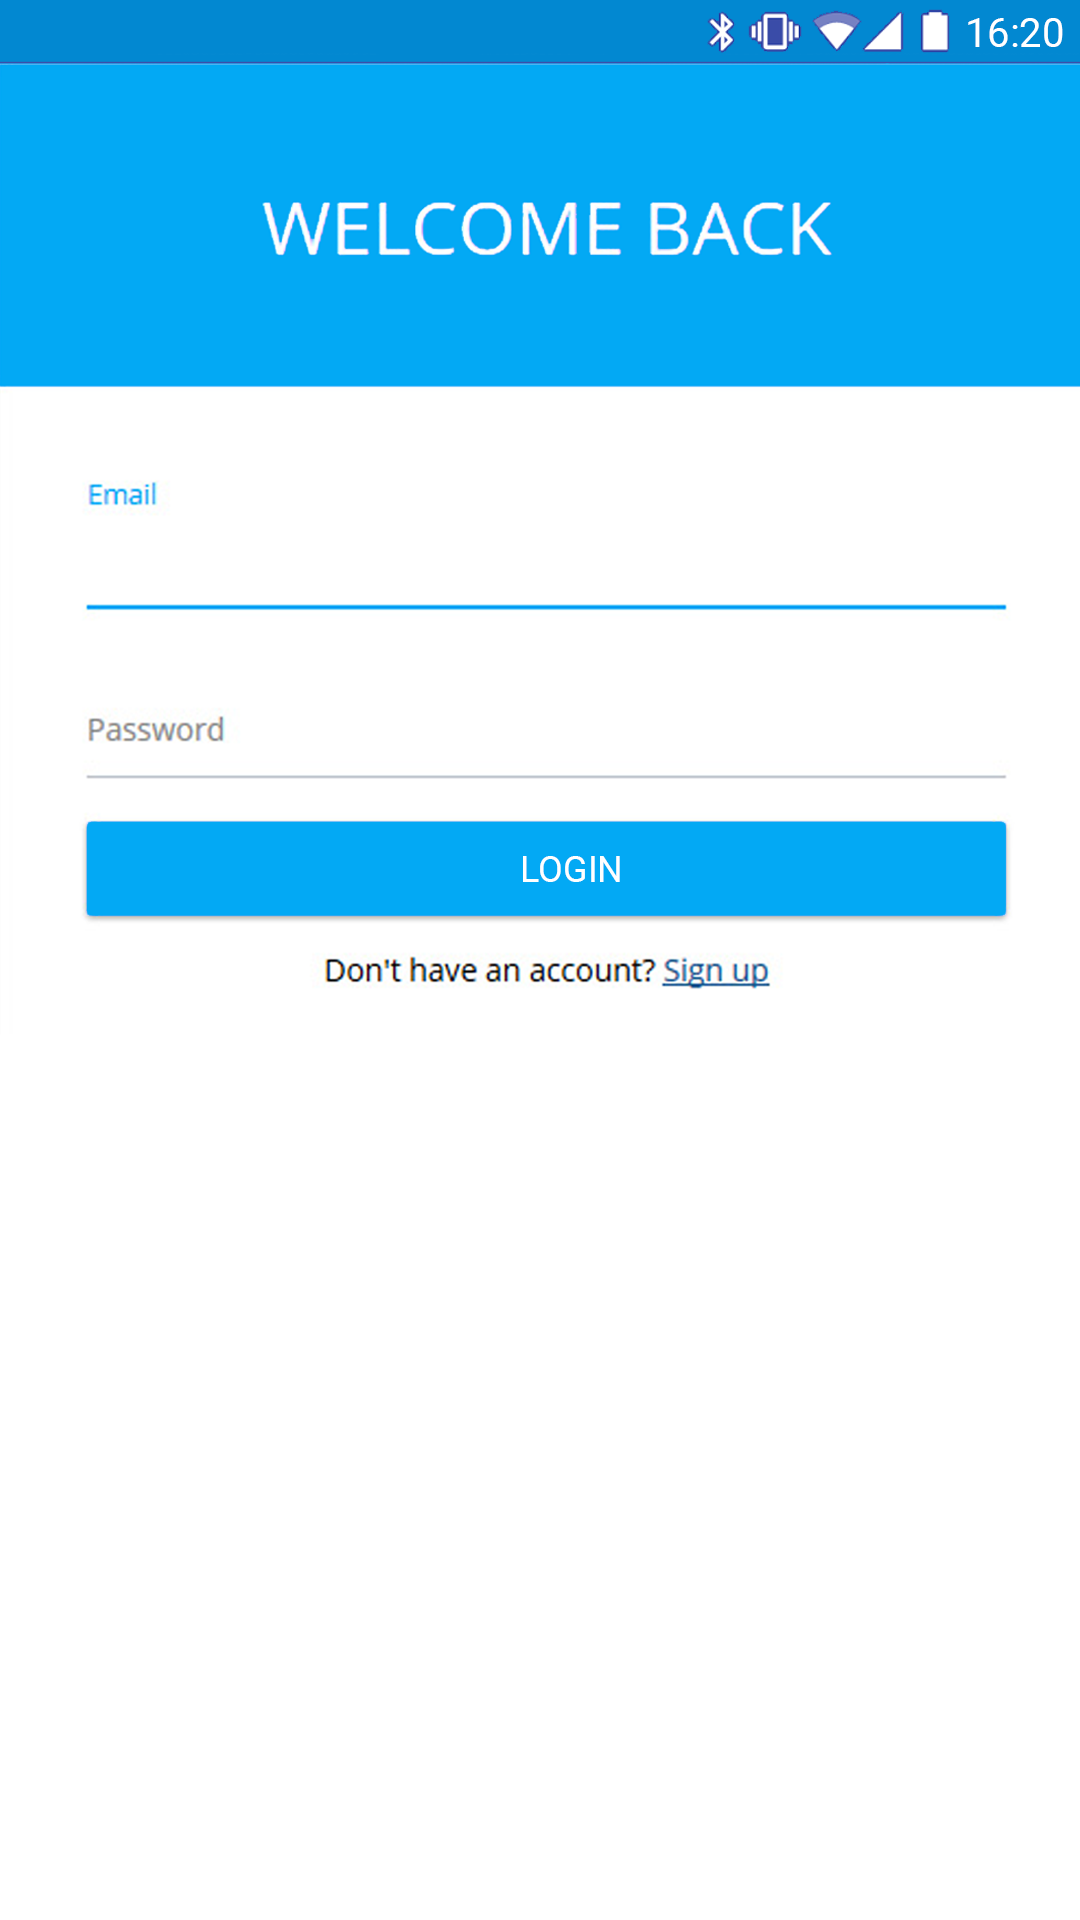
\includegraphics[width=0.9\linewidth]{manual/Login.png}
  \caption{\label{fig:vitals}The login screen}
Main screen to log into ReVA. 
   1. The login button to be clicked once all necessary information has been filled out. 
   2. The registration link that may be tapped in case users do not have an existing login. 
   3. User password input section. (Needed for verification and validation before ReVA login). 
   4. User email address input section. (Used as a username to identify users). 
\end{minipage}%
\begin{minipage}{.5\textwidth}
  \centering
  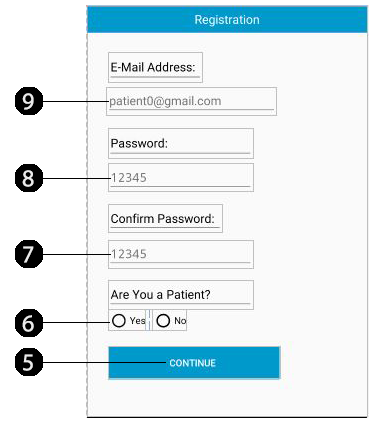
\includegraphics[width=0.9\linewidth]{manual/registration1.png}
  \caption{\label{fig:statistic}The registration screen 1}
\end{minipage}
\end{figure}
First page of registration (used by both subscribers and patients). 
  5. The continue button to proceed with the registration. 
  6. Yes/No radio button input to decide whether the user is a patient or subscriber. 
  7. Password confirmation input. 
  8. Password input for password that will be used for user login. 
  9. Email input for the email that will be used for user login. 

\begin{figure}[ht!]
\centering
\begin{minipage}{.5\textwidth}
  \centering
  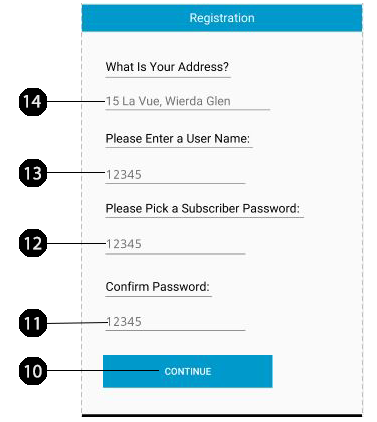
\includegraphics[width=0.9\linewidth]{manual/registration2.png}
  \caption{\label{fig:vitals}The registration screen 2}

\end{minipage}%
\begin{minipage}{.5\textwidth}
  \centering
  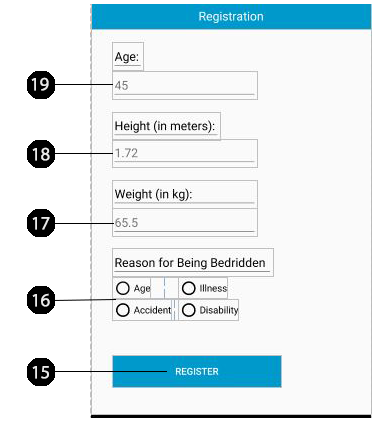
\includegraphics[width=0.9\linewidth]{manual/registration3.png}
  \caption{\label{fig:statistic}The registration screen 3}
\end{minipage}
\end{figure}

\begin{figure}[ht!]
\centering
\begin{minipage}{.5\textwidth}
  \centering
  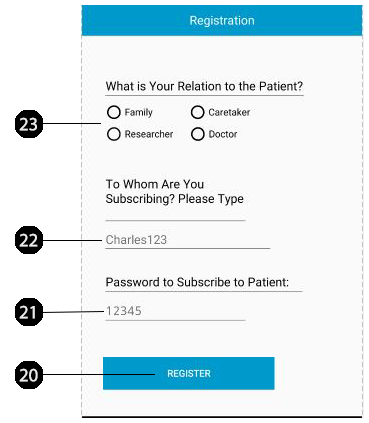
\includegraphics[width=0.9\linewidth]{manual/registration4.png}
  \caption{\label{fig:vitals}The registration screen 4}

\end{minipage}%
\begin{minipage}{.5\textwidth}
  \centering
  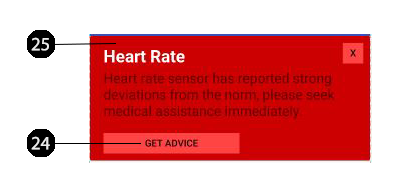
\includegraphics[width=0.9\linewidth]{manual/notification.png}
  \caption{\label{fig:statistic}The notifications screen}
\end{minipage}
\end{figure}

\begin{figure}[ht!]
\centering
\begin{minipage}{.5\textwidth}
  \centering
  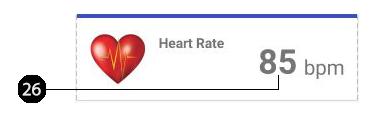
\includegraphics[width=0.9\linewidth]{manual/real-time.png}
  \caption{\label{fig:vitals}The real-time data screen 4}

\end{minipage}%
\begin{minipage}{.5\textwidth}
  \centering
  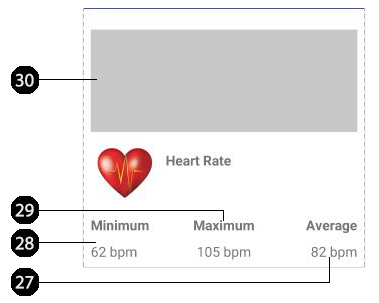
\includegraphics[width=0.9\linewidth]{manual/statistics.png}
  \caption{\label{fig:statistic}The statistics screen}
\end{minipage}
\end{figure}

%description of button and how to use it
\subsection{Patients}
%suggested format 1:
	%getting started
	You are the patient. This is all about and for you. Patients will have access to their own vitals information as well as be given the opportunity to pick their own passwords to protect said information. If a patient is unable to set up their own account with ReVA, a caretaker should assist in the process. 
	\begin{enumerate}	
	\item Logging in\\
		Patients will be prompted to log in. If a patient has an existing login, skip to step 3. 
	\item Registering\\
		If a patient does not have a login, they may follow the registration link to fill in their personal information and 			register with ReVA. Patients will have to choose their own password to login as well as a subscriber password which will 		 be used to verify subscriber validity. After they have registered, they may repeat step 1. 
	\item Logged in\\
		Now that a patient is registered and logged into the system, they may begin using it. 
	\end{enumerate}
	%using the system
	ReVA is designed to be accomodating and easy to use. Once a patient logs in, they are taken to the main screen which is comprised of two tabs: one for real time data, and the other for statistical and historical data. They may switch tabs by either swiping or tapping. See above image illustrations for more details. 
	
\subsection{Subscribers} %perhaps us a different name than subscirber.. list family member, caregiver, doctor? 
%getting started
Subscribers follow very similar steps as the patient, but they differ in that they are not required to provide additional personal information but they do have to provide a subscriber password. Since subscribers are normally caretakers (i.e. family, doctor, nurse, lover etc...) of the patient, the patient must provide them with their subscriber password so that the subscribers may subscribe to them. 
\begin{enumerate}
	\item Logging in\\
		Subscribers will be prompted to log in. If a subscriber has an existing login, skip to step 3. 
	\item Registering\\
		If no login exists for the subscriber, they may follow the registration link to register with ReVA. Once they have 			provided the necessary details and input an appropriate subscriber password, they may register. Once registered they may 		 repeat step 1. 
	\item Logged in\\
		Now that the subscriber is registered, subscribed to a patient and logged in, they may begin using the system. 
\end{enumerate}
		
	%using the system
	Subscribers have access to the real time data tab and the statistical and historical data tab. They may view both by alternating between them through tapping or swiping. See above image illustrations for more details. 

